\documentclass[12pt]{article}

%\usepackage{algo}
\usepackage{tikz,fullpage,url,amssymb,amsmath,epsfig,color,xspace,alltt,mathtools}
\usetikzlibrary{shapes,chains,positioning}
\usepackage[pdftitle={CS 240 Assignment 2},%
pdfsubject={University of Waterloo, CS 240, Fall 2021},%
pdfauthor={MP}]{hyperref}
%\RequirePackage{pstricks,pst-node,pst-tree} % draw trees, requires using xetex
\newlength{\nodeLength}
\newcommand{\Node}{A}
\newcommand{\setnode}[1]{
	\settowidth{\nodeLength}{#1}
	\renewcommand{\Node}[1]{
		\Tcircle[name=#1]{\makebox[\nodeLength]{##1}}
	}
}
\setnode{99}

\newcommand{\ceil}[1]{\left\lceil #1 \right\rceil}
\newcommand{\floor}[1]{\left\lfloor #1 \right\rfloor}
\renewcommand{\thesubsection}{Problem \arabic{subsection}}

\begin{document}
	
	\begin{center}
		{\Large\bf Problem 5}\\
		\vspace{3mm}
	\end{center}
	
	\definecolor{care}{rgb}{0,0,0}
	\def\question#1{\item[\bf #1.]}
	\def\part#1{\item[\bf #1)]}
	\newcommand{\pc}[1]{\mbox{\textbf{#1}}} % pseudocode
	
	
	
	%%%%%%%%%%%%%%%%%%%%%%%%%%%%%%%%%%%%%%%%%%%%%%%%%%%%%%%%%%%%%
	
	a)
	
	\begin{center}
		% define how to draw nodes and what distances to keep between them
		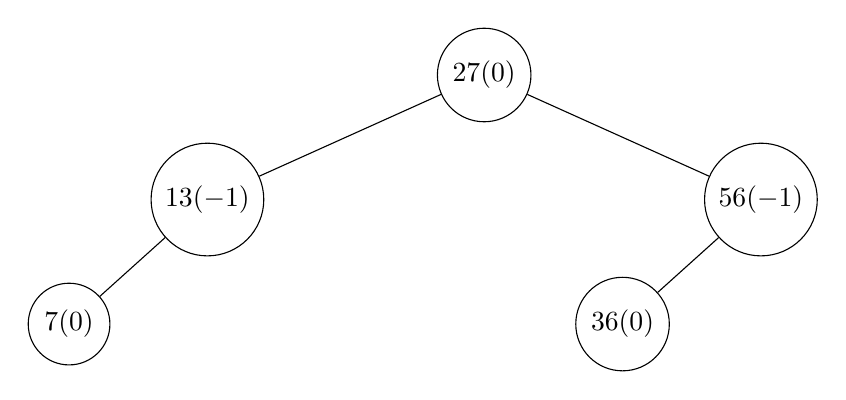
\begin{tikzpicture}[
			level distance=45 pt,
			every node/.style={circle,draw}, % nodes are circles
			level 1/.style={sibling distance=200 pt},
			level 2/.style={sibling distance=100 pt},
			level 3/.style={sibling distance=60 pt}
			]
			\node {$27(0)$}
			child {node {$13(-1)$}
				child {node {$7(0)$}}
				child [missing]
			}
			child {node {$56(-1)$}
				child {node {$36(0)$}}
				child [missing]
			};
	\end{tikzpicture}\end{center}

	\begin{center}
		% define how to draw nodes and what distances to keep between them
		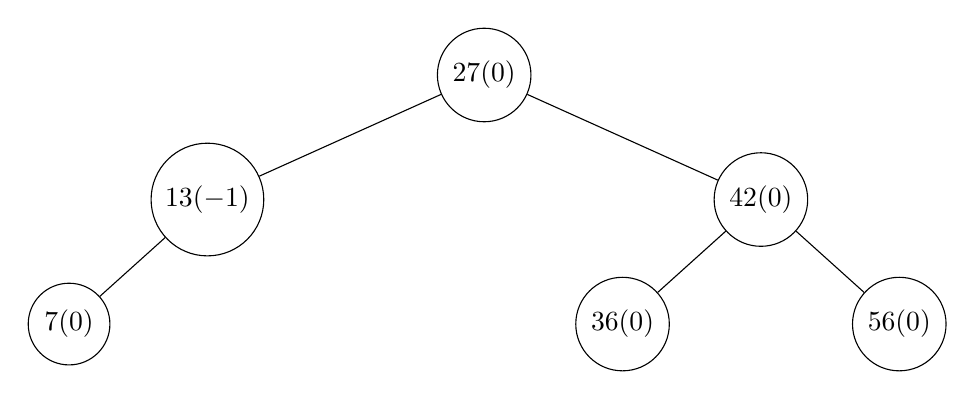
\begin{tikzpicture}[
			level distance=45 pt,
			every node/.style={circle,draw}, % nodes are circles
			level 1/.style={sibling distance=200 pt},
			level 2/.style={sibling distance=100 pt},
			level 3/.style={sibling distance=60 pt}
			]
			\node {$27(0)$}
			child {node {$13(-1)$}
				child {node {$7(0)$}}
				child [missing]
			}
			child {node {$42(0)$}
				child {node {$36(0)$}}
				child {node {$56(0)$}}
			};
	\end{tikzpicture}\end{center}
	
	
	b)
	\begin{center}
		% define how to draw nodes and what distances to keep between them
		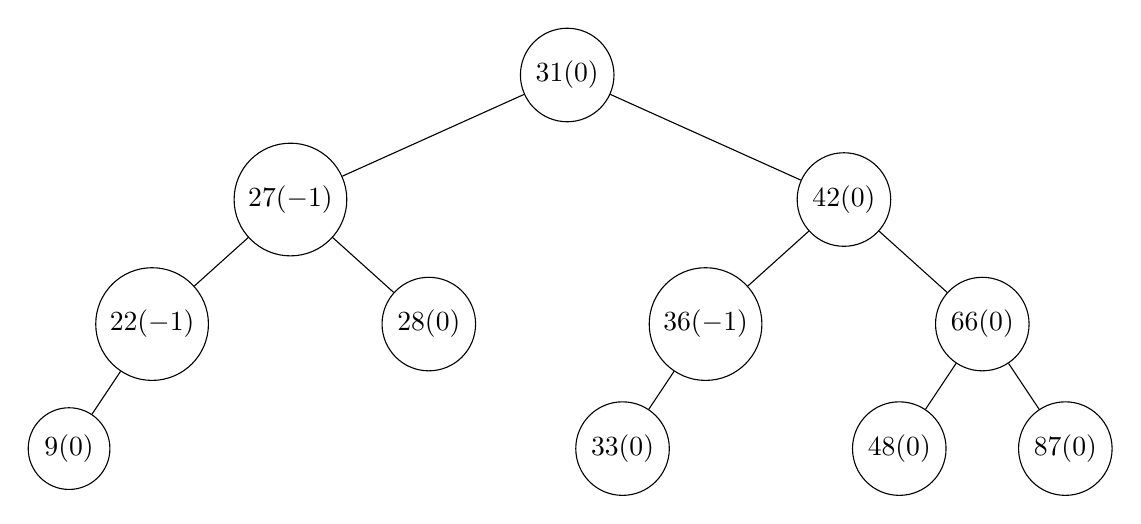
\begin{tikzpicture}[
			level distance=45 pt,
			every node/.style={circle,draw}, % nodes are circles
			level 1/.style={sibling distance=200 pt},
			level 2/.style={sibling distance=100 pt},
			level 3/.style={sibling distance=60 pt}
			]
			\node {$31(0)$}
			child {node {$27(-1)$}
				child {node {$22(-1)$}
					child {node {$9(0)$}}
					child [missing]}
				child {node {$28(0)$}}}
			child {node {$42(0)$}
				child {node {$36(-1)$}
					child {node {$33(0)$}}
					child [missing]}
				child {node {$66(0)$}
					child {node {$48(0)$}}
					child {node {$87(0)$}}}
			};
	\end{tikzpicture}\end{center}
	
	
	
	%%%%%%%%%%%%%%%%%%%%%%%%%%%%%%%%%%%%%%%%%%%%%%%%%%%%%%%%%%%%%
\end{document}